\section{\toolname Approach}
\label{sec:approach}

This section describes the current high-level design of \toolname. It is intentionally written as a structured placeholder: it captures the design choices that are already supported by the local SystemDesign documents, while leaving implementation details, optimization choices, and final algorithmic claims as \need{NEEDS METHOD DETAIL}.

\subsection{Overview}
\toolname takes as input a CVE record, the target repository, the fixing commit family, release tags, and optional CVE context such as NVD description or advisory text. It outputs a predicted set of affected release tags. The framework is organized into three stages:
\begin{enumerate}[leftmargin=*]
  \item \textbf{Step1: fix-family and patch semantic filtering.} Parse fixing commits, extract changed files and hunks, classify commit-level and chunk-level roles, and produce patch semantics for later reasoning.
  \item \textbf{Step2: root-cause vulnerability evidence extraction.} Convert patch semantics and CVE context into root-cause-level evidence, including vulnerable sequences, fix guards, scope constraints, and evidence risks.
  \item \textbf{Step3: boundary-event reconstruction and release projection.} Build release-line structure, judge boundary events, propagate vulnerability state through the Git DAG, and project affected states to release tags.
\end{enumerate}

The corpus synthesis suggests a design rule that should be preserved as the method matures: deterministic evidence preparation should reduce the search space before expensive semantic judgment. FIRE, MOVERY, ReDeBug, V1SCAN, VULTURE, and VUDDY all use staged filtering or indexing to make vulnerability search scalable~\cite{fire2024,movery2022,redebug2012,v1scan2023,vulture2025,vuddy2017}; AgentSZZ and related agent papers show that scoped tool interfaces and context compression are important for keeping LLM-based repository investigation tractable~\cite{agentszz2026,howwhyagents2026}. \toolname adopts this as a paper-level boundary: semantic judgment should be scoped to evidence-backed boundary events, while Git-DAG state propagation and release-tag projection remain deterministic.


\begin{figure*}[t]
  \centering
  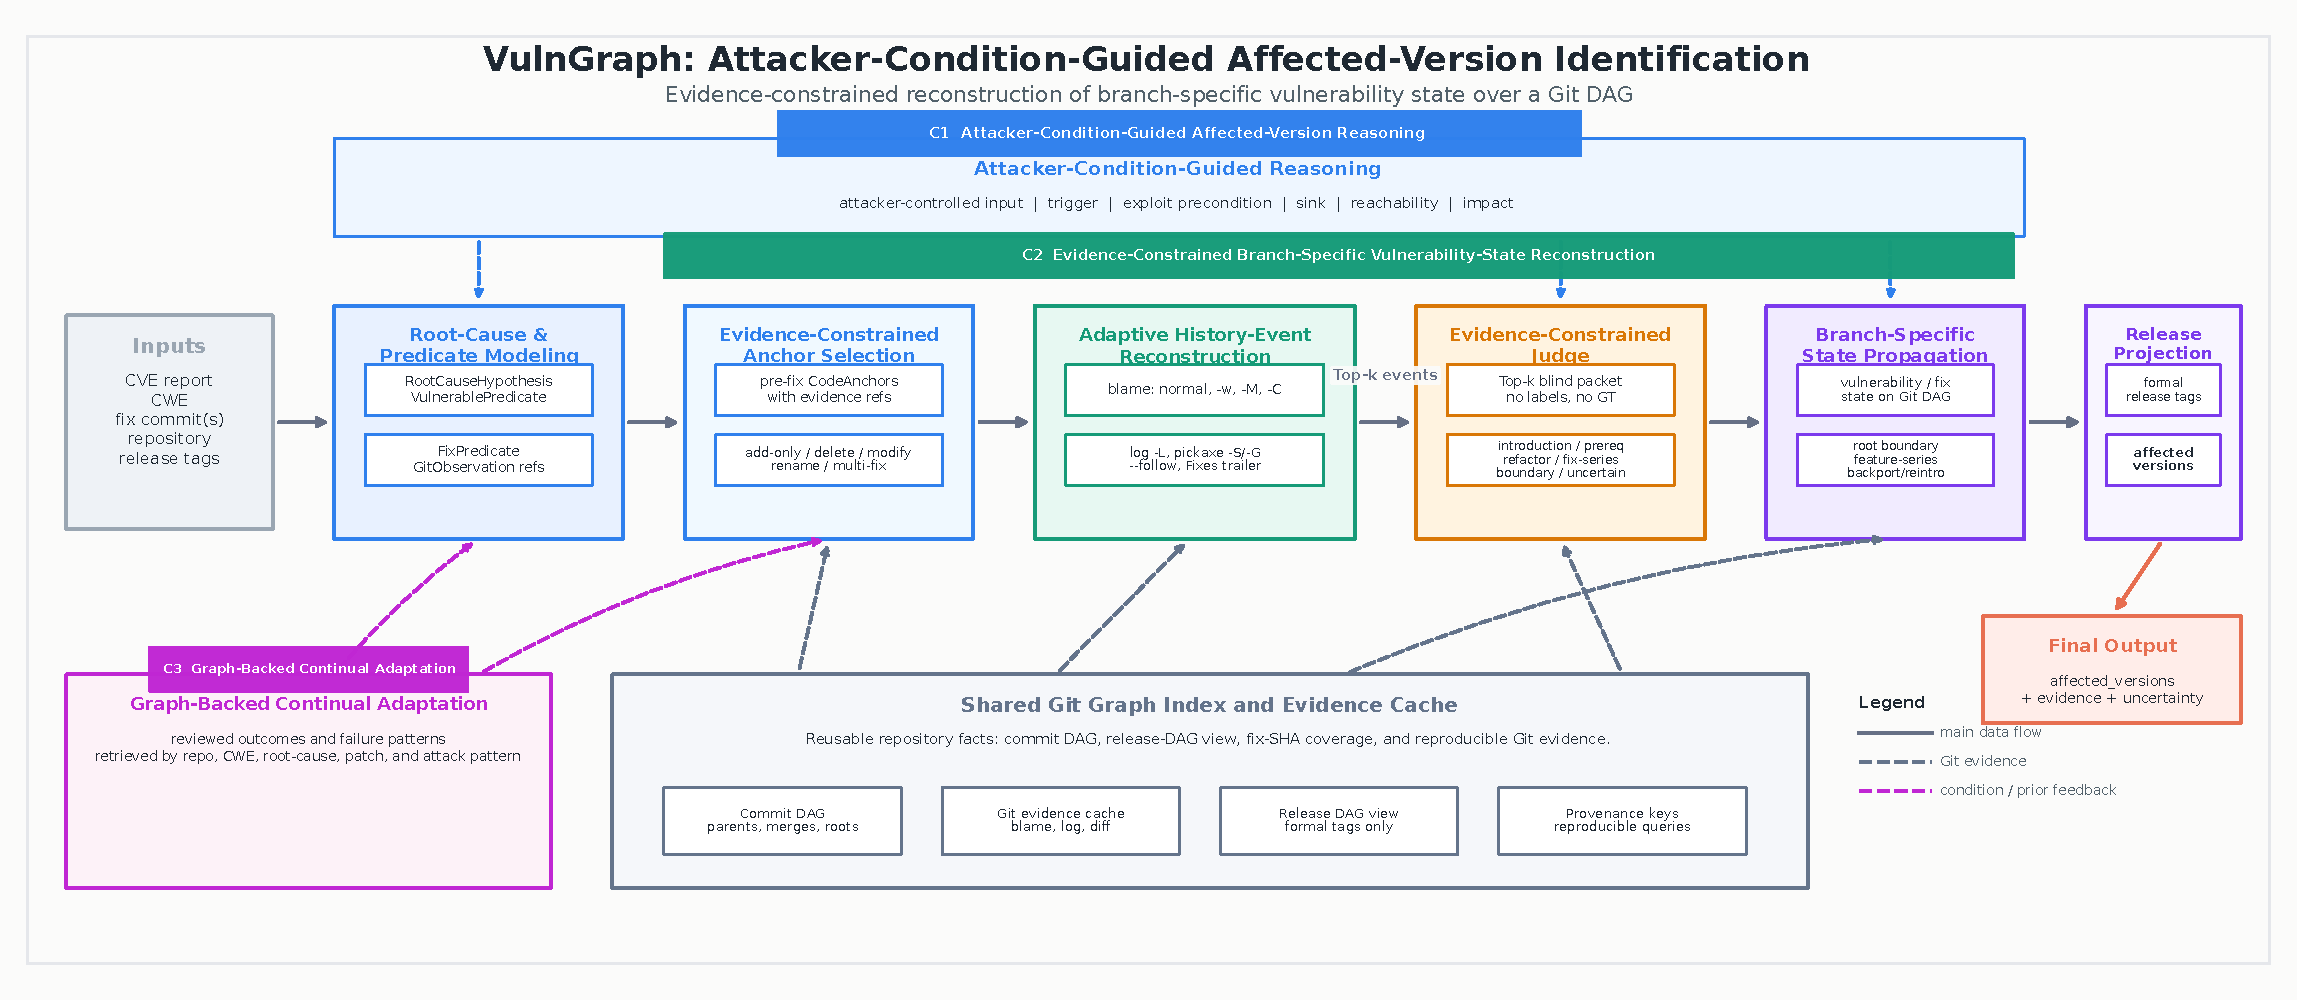
\includegraphics[width=\textwidth]{Figures/fig_vulngraph_overview.pdf}
  \caption{Overview of VulnGraph.}
  \label{fig:overview}
\end{figure*}

\subsection{Step1: Fix-Family Semantic Filtering}

The first stage exists because a CVE may map to multiple fixing commits and because each fixing commit may contain irrelevant hunks. The local design document records that the baseline dataset contains 1,128 CVEs and 1,542 patches, with 68 multi-commit CVEs after local flattening. It also records 4,783 patch chunks across the local dataset processing artifacts. These figures should be rechecked before camera-ready use \need{NEEDS EVIDENCE}.

Step1 is designed to output structured artifacts such as \texttt{fix\_family\_semantics.json}, \texttt{commit\_semantics.jsonl}, \texttt{chunk\_semantics.jsonl}, and \texttt{patch\_semantics.json}. Its role is not to decide affected versions. Instead, it provides clean, typed, and source-referenced patch evidence to Step2. In particular, Step1 should distinguish primary fixes from supporting fixes, contextual changes, tests, documentation, wrapper commits, and refactoring noise.

\subsection{Step2: Root-Cause-Level Evidence}

Step2 extracts a root-cause-level vulnerability existence theorem, abbreviated as VET in the design documents. The intended VET representation separates five concepts:
\[
\Theta = \langle S, V, F, G, C \rangle
\]
where $S$ is the vulnerability scope, $V$ is vulnerable evidence, $F$ is fix evidence, $G$ is guard or applicability constraints, and $C$ is the certificate policy. This representation is still a design placeholder \need{NEEDS METHOD DETAIL}, but it encodes an important boundary: touched files and changed lines are not automatically root-cause evidence.

Step2 should output artifacts such as \texttt{root\_cause\_vet.json}, \texttt{vet\_evidence\_graph.json}, \texttt{vet\_admission\_input.json}, and a compatibility \texttt{rci.json}. These artifacts provide the evidence packet used by Step3 for prioritizing boundary-event reconstruction.

This design is motivated by repeated warnings across the reference corpus: patch signatures, deleted lines, and cloned functions are useful evidence, but none of them alone proves that the vulnerability condition holds in a released version~\cite{vszz2022,redebug2012,vuddy2017,movery2022,vercation2026}. The VET artifact is therefore meant to make the required vulnerable condition explicit before boundary events are judged.

\subsection{Step3: Boundary Reconstruction and Release Projection}

Step3 is responsible for affected-version identification. The current main path is: fixing commits, candidate history events, boundary-event judgment, Git-DAG state propagation, and release-tag projection.
The semantic-judgment boundary is explicit: judgment is applied to candidate boundary events, while the release-line graph and release-tag projection are handled by deterministic repository analysis.

This separation is central to \toolname. Deterministic Git-DAG state propagation keeps the method auditable and cost-aware; semantic judgment is reserved for cases where boundary evidence must be interpreted. The final Step3 design still requires experimental validation before it can be presented as a complete algorithm \need{NEEDS EXPERIMENT}.

\subsection{Expected Agent Interface}

The planned semantic-judgment interface is deliberately narrow. For each candidate boundary event, the model receives scoped evidence derived from Step1 and Step2, repository snippets around the event, and a required output schema containing a selected, rejected, or uncertain judgment plus evidence references. Inspired by agentic SZZ evaluations~\cite{agentszz2026,howwhyagents2026}, \toolname should log token usage, tool calls, latency, and failure modes for every judgment. The exact prompt, tool API, and judgment schema remain \need{NEEDS METHOD DETAIL}.

\subsection{Memory and Self-Evolution Hooks}

The broader SystemDesign materials describe typed memory, verifier-gated skill evolution, and artifact promotion as future capabilities. In this draft, these are not claimed as completed experimental components. They are positioned as optional design hooks: failed boundary judgments may become failure memories, repeated repair procedures may become procedural memories, and stable verified patterns may eventually be compiled into deterministic artifacts. Any final claim about these mechanisms requires implementation and ablation evidence \need{NEEDS EXPERIMENT}.
